\documentclass[12pt]{article}
\usepackage{amsmath, amssymb, fullpage, bbm, float}
\usepackage{array}
\usepackage{graphicx,psfrag,epsf}
\usepackage{enumerate}
\usepackage{caption}
\usepackage{subcaption}
\usepackage{setspace}
\usepackage{color}
%\usepackage{natbib}
\usepackage{url} % not crucial - just used below for the URL
\renewcommand{\vec}[1]{\mathbf{#1}}

%\pdfminorversion=4
% NOTE: To produce unblinded version, replace "0" with "1" below.
\newcommand{\blind}{1}

%AGW: I just changed the margins and spacing to
%make things easier to proofread. Uncomment the following and
%comment out the doublespacing command below.
% DON'T change margins - should be 1 inch all around.
\addtolength{\oddsidemargin}{-.5in}%
\addtolength{\evensidemargin}{-.5in}%
\addtolength{\textwidth}{1in}%
\addtolength{\textheight}{-.3in}%
\addtolength{\topmargin}{-.8in}%

\begin{document}

%\bibliographystyle{natbib}

% \def\spacingset#1{\renewcommand{\baselinestretch}%
% {#1}\small\normalsize} \spacingset{1}

%%%%%%%%%%%%%%%%%%%%%%%%%%%%%%%%%%%%%%%%%%%%%%%%%%%%%%%%%%%%%%%%%%%%%%%%%%%%%%

\if1\blind
{
\title{Bayesian Modeling and Test Planning for Multi-phase Reliability Assessment}

\author{James F.\ Gilman\\North Carolina State University\\Raleigh, NC\\\texttt{jfgilman@ncsu.edu} \and
Kassandra M.\ Fronczyk\\Lawrence Livermore National Laboratory\\Livermore, CA\\\texttt{fronczyk1@llnl.gov} \and
Alyson G.\ Wilson\\North Carolina State University\\Raleigh, NC\\\texttt{agwilso2@ncsu.edu}}
\maketitle} \fi

\if0\blind
{
  \bigskip
  \bigskip
  \bigskip
  \begin{center}
    {\LARGE\bf Bayesian Modeling and Test Planning for Multi-phase Reliability Assessment}
\end{center}
  \medskip
} \fi

\bigskip

\begin{abstract}
We propose a Bayesian hierarchical model to assess the reliability of a family of vehicles, based on the development of the Joint Light Tactical Vehicle (JLTV). The proposed model effectively combines information across three phases of testing and across common vehicle components. The analysis yields estimates of failure rates for specific failure modes and vehicles as well as an overall estimate of the failure rate for the family of vehicles. We are also able to obtain estimates of how well vehicle modifications between test phases improve failure rates. In addition to using all data to improve on current assessments of reliability and reliability growth, we illustrate how to leverage the information learned from the three phases to determine appropriate specifications for subsequent testing that will demonstrate if the reliability meets a given reliability threshold.
\end{abstract}

\noindent%
{\it Keywords:}  Assurance Testing, Combining Information, Defense Acquisition, Reliability, Reliability Growth
\vfill

\newpage
\doublespacing
\section{Introduction}
Reliability is a high priority in the testing of defense systems. A common
metric is {\em reliability growth}, which tracks the change, and ideally
improvement, in the reliability of a system as it moves through testing phases
and undergoes periodic corrective actions. To most effectively use resources
plans for future test events should be based on what has been observed in
previous testing.

In this paper, we propose models for combining information across multiple test phases with
the ultimate objective of planning a future test. When combining information, there is no
omnibus solution. Rather, models need to be carefully considered and evaluated
to ensure that they accurately reflect the data and the underlying physical
processes. Our analysis is motivated by the reliability assessment of the Joint Light
Tactical Vehicle (JLTV), which is a family of vehicles designed to replace
one-third of the legacy high-mobility multipurpose wheeled vehicle (Humvee)
fleet. There are four unique types of vehicles, and within types there are many
possible variants. The primary mission of the family of vehicles is to provide
ground mobility that is deployable worldwide and capable of operating across the
range of military roles including combat, sustainment, police action,
peacekeeping, and security patrol, in all weather and terrain conditions.

The JLTV was evaluated using multiple test events as it was developed.
Engineering and Manufacturing Development (EMD) included three phases of
testing, where fixes occurred only during a set Corrective Action Period (CAP)
between each phase. For every vehicle, each failure encountered during testing
was recorded and attributed to a specific failure mode.  Since fixes were
delayed to CAPs, analysis generally shows a distinct jump in the system
reliability between test phases.

We propose a model that can effectively combine information across the three
phases of testing and across common vehicle components. We use a Bayesian
hierarchical model to assess the reliability of the family of vehicles. The
model accounts for the commonality across vehicle types and allows for
uncertainty quantification. Inferential objectives from the proposed model
include an estimate of the mean miles between failure (MMBF) for each vehicle,
failure mode, and phase of test, and an assessment of the effectiveness of the
corrections completed in the CAPs. Additionally, because future tests are being
planned, we propose methodology to leverage the information learned from the
three phases to determine the length of testing needed to demonstrate a given
reliability threshold in subsequent testing.

\section{Data}
Eight vehicle prototypes were used for reliability, availability, and maintainability (RAM) testing of the JLTV. There were four two-seat utility vehicles,
two four-seat general purpose vehicles, a two-seat heavy guns carrier, and a
two-seat close combat weapons carrier. The close combat weapons carrier, one
general purpose, and two utility vehicles were tested in Aberdeen, Maryland, and the heavy weapons carrier, one general purpose, and two utility vehicles
were tested in Yuma, Arizona. When comparing the test sites, the Maryland test site is much colder in the winter months but the terrain is not as harsh; in Arizona, it is warmer but with more challenging terrain. Using two test sites allows for the system to be tested under a broader range of environmental conditions.
The vehicles were driven roughly 3000 to 5000 miles in Phase 1, between
4500 and 7500 miles in Phase 2, and between 5000 and 6700 miles in Phase
3. The actual mileage we use in our case study has been altered to protect proprietary information.

There are many similarities between vehicle types; in fact, the most dissimilar
vehicles have over 80\% common parts. Consequently, some failure modes, such as those for
brakes and radios, will be common to all eight vehicles. Other failure modes
will be related, but not identical, as with hydraulics, frame, and body. There are 1412 observed failures attributed to 26 failure modes recorded across
all eight vehicles and all three test phases. In any given phase of test, every
vehicle is not guaranteed to have a failure of all 26 failure modes, and each
test phase does not necessarily end with a failure. Therefore, we have 624 right
censored observations, which account for miles driven after the last observed failures.

\section{Methodology}
A typical reliability analysis employed by the Department of Defense (DoD) test
community would consider each test phase independently and use the exponential
distribution to model the miles between failure for the system ~\cite{ref1}. For many situations, including our example, this
traditional analysis is overly simplistic, relying on incorrect modeling assumptions and ignoring valuable information learned about the individual vehicles and their failure modes through multiple phases of testing.

We propose an alternative approach using a Bayesian hierarchical
model.  The methodology section is organized as follows.  In Section~\ref{modrel}, we introduce a general structure that models the relationships in the
data across all test phases, while accounting for CAPs, and incorporates known
similarities between vehicle failure modes.  Next, we will consider different
distributional assumptions and their implications.  Using the JLTV as a case study we
will illustrate the process of model selection using three different diagnostic
checks.  In Section~\ref{atp} we discuss methods of designing next stage test plans.
First we outline the traditional approaches, then we propose a Bayesian
approach that allows the practitioner to leverage the information from previous test phases, using the models developed from Section~\ref{modrel}, with the hopes of reducing testing resources required while minimizing producer and consumer risks.

\subsection{Modeling Reliability}\label{modrel}
In this reliability setting, we are analyzing time to failure data measured in
miles for a multiple component system with the primary objective of
assessing the system failure rate and predicting future failure counts.
The most common models used in this kind of failure rate analysis are lifetime
distributions, and the most common for failure count analysis is the
\emph{Poisson process} family of counting models.

\subsubsection{Model Structure}
For each phase of testing we have failure mileage data for
a given vehicle $i$ and failure mode $j$ denoted as $t_{ij0}, t_{ij1},...,
t_{ijn_{ij}}, t_{ijc}$, where $t_{ij0} = 0$ and $t_{ijc}$ is the censored
observation at the end the testing phase. In each phase of testing, we assume
the vehicle miles between failures, $y_{ijk} = t_{ijk} - t_{ijk-1}$, follow a
lifetime distribution, $f(\cdot)$, with an unknown set of parameters that include
a rate parameter.  For the first phase of testing, the rate parameter for vehicle $i$ and
failure mode $j$ will be denoted as $\lambda_{ij}$.  For the next stage, we use the same $\lambda_{ij}$ but add a multiplicative correction parameter
$\rho_{j}^{P2}$ that represents the change in this rate due to the CAP.  This
procedure is then repeated for each subsequent stage.  The correction parameter
will be discussed more in the next section, but the general model is:
\begin{align*}
\text{Phase 1: }&y_{ijk}\mid\lambda_{ij}\sim f(\cdot) \\
\text{Phase 2: }&y_{ijk}\mid\lambda_{ij}\rho_{j}^{P2}\sim f(\cdot) \\
\text{Phase 3: }&y_{ijk}\mid\lambda_{ij}\rho_{j}^{P2}\rho_{j}^{P3}\sim f(\cdot) \\
\quad i = 1,2,...,v \quad &j=1,2,...,s \quad k=1,2,...,n_{ij}
\end{align*}
where $v$ represents the number of vehicles, $s$ is the number of failure modes,
and $n_{ij}$ are the number of failures of vehicle $i$ failure mode $j$.  The number of vehicles $v$ and number of failure modes $s$ are considered fixed and the same across all phases.

For the model we assume a prior distribution on the failure rate parameter
$\lambda_{ij}$.  This distribution depends on whether failure mode $j$ is
considered to be common across vehicles or related but not identical.  If
failure mode $j$ is considered common across vehicles, we will assume there is a
single failure rate $\lambda_j$ that is shared by all eight vehicles with a
prior distribution that has positive support.  In the case study, we will use a
non-informative gamma distribution.  For failure modes that are considered
related across vehicles, but that are not expected to be exactly the same, we place a
prior distribution on the collection of $\lambda_{ij}$; in other words, we
assume each of the vehicles has a distinct failure rate for failure mode $j$ but
they arise from a common distribution.  This is the common Bayesian hierarchical
modeling structure, where we then place  hyperprior distributions on the shared
distribution's parameters.  In the case study, we use a gamma distribution with
non-informative hyperpriors for all related failure modes.  Many times in
practice  it is difficult to know ahead of time if individual components should
be modeled  as common or related.  In the case study, we fit models for each
component with both model structures and use diagnostic tools  that are
discussed in Section~\ref{modd} to make our final decision.

\subsubsection{Fix Effectiveness}\label{FEF}
After the first CAP, the second test phase begins with repaired vehicles. To plan for the reliability improvement caused by
these repairs, the PM2 reliability growth model \cite{ref2} is often used.
This model explicitly captures testing phases, choices about which failure modes
to correct, and the potential of not completely eliminating a failure upon
repair. Since PM2 is used for planning, many parameters of potential
interest are assumed fixed. An example is the Fix Effectiveness Factor (FEF), which measures how much
repairs improve failure rates. A common value for FEF is
0.70. We follow the premise of this type of model, but allow a more flexible and
data-driven result.

One common assumption in reliability growth modeling is nondecreasing
failure rates: either the fixes were effective or had no effect, but did
not degrade the reliability of the family of vehicles.  This should generally be the case, but
because we are dealing with complex systems and testing conditions are rarely
completely consistent, we will sometimes see decreases in failure rates after repairs are made.  Thus we choose a prior distribution for the
FEF parameter $\rho_{j}^{P2}$ that has positive support.  If
$\rho_{j}^{P2}$ is less than one, this represents an improvement in reliability.
The same approach is applied to $\rho_{j}^{P3}$ for the correction period
between phases two and three.  With this structure we can use the posterior
distributions of the correction parameters to make inference on the effectiveness
of the repairs and the joint posterior distributions to evaluate the overall system reliability within each phase.

\subsubsection{Distributional Assumption}
The next modeling choice that must be made is selecting an appropriate
probability model. This includes a selecting a sampling distribution for the data
and prior distributions for each parameter on which the sampling distribution
depends. Some common distributional choices for lifetime data are exponential, Weibull, lognormal, gamma, inverse
Gaussian, and normal failure time models.  Because all of these distributions
have a rate parameter (sometimes called a scale parameter, which is the reciprocal of the rate parameter), they can be applied in
the proposed modeling structure. We focus on the
exponential and Weibull distributions, which are commonly used for reliability.

The exponential model has probability density function
\begin{equation*}
    f(y_{ijk}|\lambda_{ij})=\lambda_{ij} \exp(-\lambda_{ij}y_{ijk}) \;.
\end{equation*}

This is by far the most common parametric distribution used in reliability
modeling because of its desirable mathematical properties and straightforward interpretations.  One convenient property, because we are assuming
independence between failure modes, is that the overall system failures also follow
an exponential distribution with a system failure rate $\lambda_S =
\sum_{j}\lambda_{j}$.  A second, potentially less attractive property, is that the hazard rate is constant over miles.  For the case study, this implies that a given
component is equally likely to fail in the first mile of testing as it is in the thousandth.  This may be reasonable for some components, but in many settings we observe either a decreasing hazard rate, where failures are likely to
occur early in testing but less likely as the test goes on, or an increasing hazard rate, where we see the system wear down as the test progresses.

Despite its common use, the assumption of a constant hazard rate over time is rarely justifiable. The issues that arise when the modeling assumptions for the exponential distribution are violated are well-documented ~\cite{ref3}. Therefore, we will also consider more flexible distributions when analyzing the data.  In our analysis of the case study, we also fit the same hierarchical model structure using the Weibull as our
lifetime distribution, $f(\cdot)$. We assume that the failure mileage $t_{ijk}$ each follow a $Weibull(\lambda, \gamma)$ distribution with scale
parameter $\lambda$ and shape parameter $\gamma$, with probability density
function,
\begin{equation*}
    f(t_{ijk}|\lambda_{ij},\gamma_{i})=\lambda_{ij}\gamma_{i}
    t_{ijk}^{\gamma_{i}-1}\exp(-\lambda_{ij} t_{ijk}^{\gamma_{i}}).
\end{equation*}
The exponential is a special case of the Weibull, when $\gamma = 1$.

When a failure occurs during a testing phase, the mileage is recorded and the system is restored to full operation, often by repairing or replacing a component.  One must consider how these changes will affect the system reliability moving forward.  In repairable system literature, two common modeling assumptions are the extreme cases ``good as new" or ``bad as old".  ``Good as new" assumes that a repaired component has returned to a brand-new state or, in our case, that the mileage is set to zero.  On the other hand, ``bad as old" assumes the component has returned to the state it was at before the failure occurred.  The Weibull distribution implies we assuming ``bad as old" intra-test repairs by modeling the actual failure mileage $t_{ijk}$ instead of the miles between failures $y_{ijk}$.  This distinction is important in the Weibull case because the failure rate is not constant in time.  In the JLTV case study we have assumed ``bad as old" intra-test repairs based on input from subject matter experts.  There will be applications where repairs should be treated as somewhere between ``good as new" and ``bad as old".  This requires more complex modeling that is beyond the scope of this paper.  An overview of Bayesian approaches for repairable system models can be found in Hamada et al. ~\cite{ref4}

We index both $\rho$ and
$\gamma$ only by $j$ and not $i$. In other words, we are assuming a single
shape and between phase adjustment parameter for each failure mode across
vehicles.  All of these parameters could also be indexed by $i$ and modeled
hierarchically or we could use a combination of common and ``related".  When failure modes do not occur within the testing period, resulting in a single censored observation, this can lead to convergence issues.  In the case study, we found 6 of the 26 failure modes had less than 10 observed (non-censored) failures across all 3 phase and 8 vehicle types.  These failure modes were attributed to system components such as the engine and armor.  To improve convergence we have binned these rare failure modes into a single ``other" failure mode.  This may also be useful for planning future testing to account for previously unobserved failure modes.

\subsubsection{Model Diagnostics}\label{modd}
The decision about which model to
use can have a substantial impact on reliability assessment.  We consider a
few  goodness-of-fit techniques that can be used to help with this decision for Bayesian reliability models.  The
first model selection question we consider is the parametric form,
exponential versus Weibull.  This an example of the classic statistical modeling
the trade-off between fit and interpretability.  Because the Weibull is a more
flexible model, containing the exponential as a special case, it will always fit the data at least as well as the exponential.

The first diagnostic we use to decide between the exponential and Weibull models is
to fit the Weibull model and look at the posterior distributions of the shape
parameters to determine whether their support contains 1. From Figure~\ref{Shape}, which shows the Weibull model fits for the case study for each failure mode, we see that 1 is not a reasonable value for any of the failure modes, which suggests that the exponential model may not fit this data well.

We also consider a more formal diagnostic tool, the deviance information criterion (DIC)
~\cite{ref5}. This is a popular method for comparing the goodness of fit of
multiple models. The DIC method includes a penalty term that grows with the
numbers of unknown parameters in the model.  The DIC is unitless, with smaller values indicating a better fit to the data.  Table~\ref{table:ta1} shows the DIC results for the different distribution and structure combinations we considered for the case study. The results show that the hierarchical Weibull model fits the data much better than the exponential or common rate models.

In general, information criteria
comparisons do not tell us if the model is truly a good representation of the
underlying process -- they only compare models. The final model diagnostics method we present is called
posterior predictive checking ~\cite{ref6}.  We start with important
features of the data that we would expect to see if the experiment was repeated.
These are usually provided by practitioner with knowledge about the random
process being studied. In the case study, one feature of interest is the count of miles between failure observations less than 140 miles, for a given vehicle and phase.

We used the final exponential and Weibull models with the lowest DIC to simulate 5,000 new datasets for vehicles tested over the same number of miles for each of the three phases. We plot the resulting distributions for each of the 8 vehicles for all 3 phases. Figure~\ref{fig:test} shows two examples of the boxplots produced for one of the vehicle types, one plot from the exponential model
(left) and one plot from the Weibull model (right), with the dashed line showing
where the value from the observed dataset fell. If the model fits reasonably well, we expect to see the value from the observed data falling within the support of the simulated data. This suggests that the Weibull model fits the case study data better than the exponential data.

\subsubsection{Case Study Results}
We have introduced several models structures and distributional assumptions that accompany them.  Using Markov chain Monte Carlo (MCMC), we fit each of these models to the JLTV case study
dataset. (Details of the likelihoods and full conditional distributions are available in the appendix.) We use the posterior distributions to estimate reliability-related quantities of interest for each of the eight vehicle types.  We are able to examine a number of different summaries related to reliability at both the component and system level.

In this study, one quantity of interest is mean miles to failure (MMTF). This is different than the commonly used mean miles between failures (MMBF).  Due to the failure rate changing over time in the Weibull case MMBF depends on how many miles the vehicle is driven.  MMTF can be thought of as the average time until the first failure occurs. Figure~\ref{fig:MMTF Results} shows box plots and summary statistics from the posterior distributions of the expected miles to first failure for one of the vehicle types for each of the three phases using the exponential model (left) and the more general Weibull model (right).

Figure~\ref{fig:MMTF Results} shows that the posterior MMTF distributions from the Weibull model consistently have wider uncertainty intervals and larger means and medians than the exponential.  We saw this across all eight vehicle types.  This is a good illustration of how the choice of model can impact the final inference.

Figure~\ref{fig:CAP} shows the posterior distributions for each of the CAP parameters $\rho_{j}^{P2}$ and $\rho_{j}^{P3}$ for the hierarchical Weibull model.  These parameters were introduced in Section~\ref{FEF}.  They are multiplicative parameters added in between phases to capture the change in failure rate due to improvements by the producer.  Values less than one indicate a decrease in failure rate. Interestingly, the distributions have most of their mass close to the commonly used FEF value of 0.70.  We notice a trend of more improvement in the second CAP between phase two and three as compared to the first CAP between phase one and two.

\subsection{Assurance Test Planning}\label{atp}
In addition to fitting the data from the three phases of testing, we also want to use the reliability models to
develop plans for future testing. The objective is to demonstrate, at a desired level of confidence, that the system will meet or exceed a specified requirement. The methods to be employed will be similar to the assurance testing
as discussed by Hamada et al. ~\cite{ref4}.
Meeker and Escobar
~\cite{ref7} describe the difference between assurance testing and the more traditional
\emph{reliability demonstration test}: an assurance
test plan incorporates supplementary data and information, where the demonstration test uses only data from the current test.

In most test planning settings we are interested in controlling error rates
while minimizing the resources required for testing.  In a typical DoD acquisition
process, the error rates are referenced in terms of risk. \emph{Consumer's
risk} is the probability of purchasing a product that does not meet
reliability requirements.  \emph{Producer's risk} is the probability that a
product with acceptable reliability fails a given test.

In the case study, we determine how many miles on test $T$, are required and how many system failures to allow $c$, before the product is considered unacceptable.  We define $W(t)$ as a random variable that represents the total number of system failures after $t$ miles.  We let $\pi$ denote a system reliability-related
quantity of interest at a given time.

It is common to base both classical and Bayesian test plans on two specified levels
of $\pi$: $\pi_0$, an \emph{acceptable reliability level} (ARL), and $\pi_1$, a
\emph{rejectable reliability level} (RRL), where $\pi_1 \leq  \pi_0$. The precise definition of ARL and RRL differ between the classical and Bayesian test criteria and will be described below.

\subsubsection{Classical Approach}\label{sec321:ca}
In the classical (frequentist) test planning setting the risk criteria
are as follows. The \emph{producer's risk} is defined as the probability of
failing the test under the null hypothesis $\pi = \pi_0$, and the
\emph{consumer's risk} is defined as the probability of passing the test under an
alternative hypothesis $\pi = \pi_1$.  Suppose that we specify a maximum value,
$\alpha_c$, of the producer's risk and a maximum value, $\beta_c$, of the consumer's
risk. For test planning, these criteria become
$$
\begin{aligned}
	\text{Producer's Risk} &= P \text{(Test Is Failed } \vert \pi_0 \text{)} \\ &=
	P \text{(} W(t) > c \vert \pi_0 \text{)} \leq \alpha_c
\end{aligned}
$$
and
$$
\begin{aligned}
	\text{Consumer's Risk} &= P \text{(Test Is Passed } \vert \pi_1 \text{)} \\ &=
	P \text{(} W(t) \leq c \vert \pi_1 \text{)} \leq \beta_c
\end{aligned}
$$
To choose a test plan for specified values of $(\alpha, \pi_0, \beta, \pi_1)$,
we assume a distributional form that defines the relationship between the number
of system failures $W(t)$ and the reliability $\pi$.  We then find
the combinations of time on test and allowed failures that satisfy the risk constraints by simultaneously solving these two equations.  In the case where the component failure times are assumed to be exponentially distributed with rate parameter $\lambda_i$, the failure counts for
each component come from a homogeneous Poisson process $w_i(t) \sim
\text{Poisson}(\lambda_i t)$, and the system failure counts from $W(t) \sim
\text{Poisson}(\lambda_S t)$.  Numerous textbooks (e.g., \cite{ref8}) provide additional details of
this classical test planning approach.

\subsubsection{Bayesian Approach}
The non-Bayesian methods for determining the testing procedure rely only on distributional assumptions or asymptotic results. With a Bayesian approach, we
incorporate the supplementary data from the previous testing phases with the
hopes of minimizing the resources needed for additional testing.

We consider fully Bayesian posterior risks, which provides a
different interpretation from the corresponding classical risks.  While the classical approach
provides assurance that satisfactory devices will pass the test and that
unsatisfactory devices will fail it, posterior risks provide precisely the
assurance that practitioners often desire: if the test is passed, then the
consumer desires a maximum probability $\beta_b$ that the true reliability is less than the rejectable level, $\pi \leq \pi_1$. On the
other hand, if the test is failed, then the producer desires a maximum
probability $\alpha_b$ the true reliability is greater than the acceptable level, that $\pi \geq \pi_0$. Notice these posterior risks are fully Bayesian in the sense that they are probability statements about $\pi$.

For a test that fails, the \emph{posterior producer's risk} is the probability
that $\pi \geq \pi_{0}$, or $P \text{(}\pi \ge \pi_0 \vert \text{Test Is
Failed)}$. Notice that this is simply the posterior probability that $\pi \ge
\pi_0$ given that we have observed more than $c$ failures. In the exponential
case, if we let $\pi$ be the system failure rate $\lambda_S$ and $\pi_0$ be
predetermined acceptable failure rate $\lambda_0$, then using Bayes' Theorem,
and assuming a maximum allowable posterior producer's risk $\alpha_b$, an
expression for the posterior producer's risk for the exponential test plan
$(T,c)$ is
$$
\begin{aligned}
    P(\lambda_S \geq \lambda_0 \; \vert \; \text{Test Is Failed)} &= P(\lambda_S
    \geq \lambda_0 \; \vert \; W > c) \\ &= \int_{\lambda_0}^{\infty}
    p(\lambda_S \; \vert W > c) d\lambda_S \\ &= \int_{\lambda_0}^{\infty}
    \frac{f(W > c \vert \lambda_S)}{\int_{0}^{\infty} f(W > c \vert \lambda_S)
    d\lambda_S} d\lambda_S \\ &= \frac{\int_{\lambda_0}^{\infty} 1 - [ \sum_{W=0}^c
    \frac{(\lambda_S T)^W \exp(-\lambda_S T)}{W!}]p(\lambda_S)d\lambda_S}
    {\int_{0}^{\infty} 1 - [ \sum_{W=0}^c \frac{(\lambda_S T)^W \exp(-\lambda_S
    T)}{W!}]p(\lambda_S)d\lambda_S} \leq \alpha_b
\end{aligned}
$$
\\
\\
For simplicity, if we set $c = 0$ and then perform Monte Carlo integration
using $N$ posterior draws $ \lambda_S^{(j)} $
$$
\begin{aligned}
	 P(\lambda_S \geq \lambda_0 \; \vert \; W = 0) &=
	 \frac{\int_{\lambda_0}^{\infty} 1 - \exp(-\lambda_S T)p(\lambda_S)d\lambda_S}
	 {\int_{0}^{\infty} 1 - \exp(-\lambda_S T)p(\lambda_S)d\lambda_S} \\ &\approx
	 \frac{\sum_{j = 1}^{N} 1 - \exp(-\lambda_S^{(j)} T)I(\lambda_S^{(j)} \geq
	 \lambda_0)} {\sum_{j = 1}^{N} 1 - \exp(-\lambda_S^{(j)} T)} \end{aligned}
$$

Similarly, given that the test is passed, the \emph{posterior consumer's risk}
is the probability that $\pi \leq \pi_1$, or $P \text{(}\pi \leq \pi_0 \vert
\text{Test Is Passed)}$.  Let $\pi_1$ be a predetermined rejectable
failure rate $\lambda_1$. Assuming a maximum allowable posterior consumer's
risk $\beta_b$, an expression for the posterior producer's risk for the
exponential test plan $(T,c)$ is

$$
\begin{aligned}
    P(\lambda_S \leq \lambda_1 \; \vert \; \text{Test Is Passed)} &= P(\lambda_S
    \leq \lambda_1 \; \vert \; W \leq c) \\ &= \int_{0}^{\lambda_1} p(\lambda_S \;
    \vert W > c) d\lambda_S \\ &= \int_{0}^{\lambda_1} \frac{f(W > c \vert
    \lambda_S)}{\int_{0}^{\infty} f(W > c \vert \lambda_S) d\lambda_S} d\lambda_S \\ &=
    \frac{\int_{0}^{\lambda_1} [ \sum_{W=0}^c \frac{(\lambda_S T)^W
    \exp(-\lambda_S T)}{W!}]p(\lambda_S)d\lambda_S} {\int_{0}^{\infty} [
    \sum_{W=0}^c \frac{(\lambda_S T)^W \exp(-\lambda_S
    T)}{W!}]p(\lambda_S)d\lambda_S} \leq \beta
\end{aligned}
$$
\\
\\
For simplicity, if we fix $c = 0$ and then perform Monte Carlo integration
using $N$ posterior draws $ \lambda_S^{(j)} $ $$
\begin{aligned}
	 P(\lambda_S \leq \lambda_1 \; \vert \; W = 0) &= \frac{\int_{0}^{\lambda_1}
	 \exp(-\lambda_S T)p(\lambda_S)d\lambda_S} {\int_{0}^{\infty} \exp(-\lambda_S
	 T)p(\lambda_S)d\lambda_S} \\ &\approx \frac{\sum_{j = 1}^{N}
	 \exp(-\lambda_S^{(j)} T)I(\lambda_S^{(j)} \leq \lambda_1)} {\sum_{j = 1}^{N}
	 \exp(-\lambda_S^{(j)} T)}
\end{aligned}
$$

\subsubsection{Weibull Case}
In the exponential case, we defined our reliability quantity of interest $\pi$ as the system failure rate
$\lambda_S$.  Assuming an exponential lifetime distribution gave us a convenient distributional
form for our system failure counts with $W(t) \sim \text{Poisson}(\lambda_S t)$.

When we assume the miles to failure for each system component follow a Weibull
distribution, the system failure counts no longer follow a homogeneous Poisson
process.  When assuming ``bad as old" intra-test repairs, as described in Section 3.1.3, we find that the
failure count for a given failure mode follows a nonhomogeneous Poisson
process, $w_i(t) \sim \text{Poisson}( \lambda_i t_i^{\gamma_i} )$.  The system
failure counts for a given mileage $t$ have distribution $W(t) \sim
\text{Poisson}(\sum_i (\lambda_i t_i)^{\gamma_i})$.  In this case, the acceptable
and rejectable parameters $\pi_0$ and $\pi_1$ become quantities related to
$\lambda^* = \sum_i (\lambda_i t_i)^{\gamma_i}$.  This leads to integration that is analytically intractable, but Monte Carlo integration
allows our evaluation of the posterior producer's risk for the Weibull test plan
$(T,c)$:

$$
\begin{aligned}
	 P(\lambda^* \geq \pi_0 \; \vert \; W = 0) &= \frac{
	 \int_{\pi_0}^{\infty} 1 - \exp(- \sum_i \gamma_i \lambda_i
	 T^{\gamma_i})p(\vec{\lambda}) p(\vec{\gamma}) d\vec{\lambda}
	 d\vec{\gamma}} {\int_{0}^{\infty} 1 - \exp(- \sum_i \gamma_i \lambda_i
	 T^{\gamma_i})p(\vec{\lambda}) p(\vec{\gamma}) d\vec{\lambda}
	 d\vec{\gamma}} \\
   &\approx \frac{\sum_{j = 1}^{N} 1 - \exp(-\sum_i \gamma_i^{(j)}
   \lambda_i^{(j)} T^{\gamma_i^{(j)}}) I(\lambda^* \geq \pi_0)} {\sum_{j = 1}^{N} 1 - \exp(- \sum_i
   \gamma_i^{(j)} \lambda_i^{(j)} T^{\gamma_i^{(j)}})}
\end{aligned}
$$
\\
where $\vec{\lambda}$ and $\vec{\gamma}$ denote the vectors of $\lambda_i$ and $\gamma_i$. Again we set $c = 0$ and use $N$ posterior draws for both $\lambda_i^{(j)}$ and
$\gamma_i^{(j)}$.

It should be noted that in this test planning process, the practitioner would use
the posterior distribution of the rate parameters from the final developmental
testing phase $\lambda_i\rho^{P2}\rho^{P3}$.  It is also common to incorporate a
degradation factor to account for an expected reduction in reliability from the
developmental phase to the operational phase.  In the Bayesian framework, this
entails adding another multiplicative parameter to the rate parameter with an
appropriate prior.   A 10-30 percent reduction from the developmental phase to
the operational phase would be a common assumption in many DoD applications.

\subsubsection{Case Study Test Plan Results}
The first step in applying the Bayesian assurance test planning method to our case study is defining $\pi_0$,
$\pi_1$, $\alpha_b$ and $\beta_b$, which are the ARL, RRL, acceptable producer risk
and acceptable consumer risk respectively.  With input from subject matter
experts,  we will define the producer's target as the average number of
failures in the first 10,000 miles to be less than 155, and the consumer's minimum
requirements as the average number of failures in the first 10,000 miles to
greater than 175. The producer's targets and consumer's minimum requirements represent our cut off levels ARL and RRL respectively.  This means if the true average number of failures in the first 10,000 miles is less than 155 the producer would expect his product to fail the test a small proportion of the time, $\alpha_b$.  On the other hand, if the true average number of failures in the first 10,000 miles is greater than 175 the consumer would expect the product to pass the test a small proportion of the time, $\beta_b$. We will use $\alpha_b = 0.1$ and $\beta_b = 0.05$, and in practice these values should always be set based on
the true risk tolerances of the consumer and producers.  This gives us the
following probability statements to satisfy when designing the test:
\\
$$
\begin{aligned}
  \text{Consumer Risk} &: P(\sum_i 10,000^{\gamma_i} \lambda_i \geq 175 \; \vert \text{Test Is Passed}) \leq 0.1  \\
  \text{Producer Risk} &: P(\sum_i 10,000^{\gamma_i} \lambda_i \leq 155 \; \vert \; \text{Test Is Failed}) \leq 0.05
\end{aligned}
$$

From here we are able to find combinations of failures allowed and test miles
required that satisfy both risk requirements.

Table 2 compares the resulting test plans of our proposed method to the classical method. In general, we warn against making this comparison of test plans, because as we discuss below, each method makes different assumptions and the test plan probability constraints are addresses different questions.

As is common in DoD test planning, for the classical case we only controlled for the consumer's risk, not for both risks as described in Section~\ref{sec321:ca}. Notice this leads to extremely high levels of producer risk under the classical plan. (Note that with the proposed values of  $\pi_0$, $\pi_1$, $\alpha_c$ and allowed failures there was no test mileage that would satisfy both classical risk criteria.) The classical plan assumes product is either acceptable or unacceptable and then controls the probability of error in each of those cases. For example, interpreting the first row of Table 1, if a system is put on test where the average number of failures in 10,000 miles is 155, the the probability of failing the test and observing two or more failures in 225 miles is 0.86. If a system is put on test where the average number of failures in 10,000 miles is 175, then the probability of passing the test and observing no more than one failure in 225 miles is 0.10.

By comparison, the Bayesian plan puts constraints on the probability of error when the test is passed and failed.  From the study, the posterior producer risk is the probability the average number of failures in 10,000 miles for the system is less than 155 given that the test is failed and two or more failures are observed in 240 miles. The posterior consumers risk is the probability that the average number of failures in 10,000 miles for the system is greater than 175 given that the test is passed by observing no more than one failure in 240 miles.

We have provided one example where there was no solution that satisfied all of the constraints using the classical method.
This problem does not only come up using the classical method.  Both test planning approaches rely heavily on setting reasonable values for $\pi_0$, $\pi_1$, $\alpha$ and $\beta$.   When these are set to unrealistic values both procedures can result in no plan that satisfies the probability statements ~\cite{ref9}.

In this paper we have focused on test plans for single units, but the assurance testing methodology can be extended to find test plans that
allow for a changing number of testing units.  In this case you would find
combinations of failures allowed and test miles required and number of vehicles
tested that satisfy the risk requirements. More details and examples of this can
be found in Hamada et al. ~\cite{ref4}

\subsection{Discussion}
The JLTV results provide indications that our model is successfully
capturing the failure rates across failure modes, inferring logical fix
effectiveness factor distributions, and providing reliability estimates that can
be leveraged for future test planning. In the traditional analysis, we do not
typically look at failure rates of the failure modes, nor would we be able to
leverage the commonalities across vehicles. The proposed modeling framework
overcomes these limitations and allows for more realistic reliability estimates
for vehicles with no observed failures. Additionally, our data-driven approach
for reliability growth improves on the current growth models being used in the
DoD, which are based solely on fixed quantities set by management.

While our basic approach provides reasonable initial inferences, there are
several extensions to incorporate. For example, reliability estimates for
vehicles with no observed failures are sensible; however, we should leverage
more information across vehicles. Because our
current model assumes independence across failure modes, potential methods that model the correlation structure
between failure modes are being investigated. We
also need to look more closely at the intra-phase repair assumptions.  Applying
repairable system methodology in the modeling and reliability assessment stage
could be a good approach, but this could  add a great deal of complexity to the
assurance planning stage.


%%%%% ref %%%%%%%%%%%%%%%%%%%%%%%%%%%%%%%%%%%%%%%%%%%%%%
\begin{thebibliography}{99}
\bibitem{ref1} Director, Defense Test and Evaluation. Test and evaluation of system reliability availability maintainability - A primer; Third Edition 1982. \url{http://www.dtic.mil/dtic/tr/fulltext/u2/a120261.pdf}
\bibitem{ref2} P.\ M.\ Ellner, J.\ B.\ Hall. An approach to reliability
growth planning based on failure mode discovery and correction using AMSAA
projection methodology. \textit{Proceedings of the Annual Reliability and
Maintainability Symposium} 2006.
\bibitem{ref3} National Research Council. Statistics, Testing, and Defense
Acquisition: Background Papers. \textit{National Academies Press} 1999.
\bibitem{ref4} M.\ Hamada, A.\  Wilson, C.\ Reese, H.\ Martz. Bayesian Reliability. Springer 2008.
\bibitem{ref5} D.\  Spiegelhalter, N.\ Best, B.\ Carlin, A.\ Van der
Linde Bayesian measures of model complexity and fit. \textit{Journal of the Royal Statistical
Society, Series B}, 64: 583-640 2002.
\bibitem{ref6} A. Gelman, M. Xiao-Li, H. Stern. Posterior predictive assessment of model fitness via realized discrepancies (with discussion). \textit{Statistica Sinica} 6, 733-807 1996.
\bibitem{ref7} W.\ Meeker, L.\ Escobar. Reliability: the other
dimension of quailty. \textit{Quality Technology and Quantitative Management} 1, 1-25 2004.
\bibitem{ref8} J.\ F.\ Lawless. Statistical Models and Methods for Lifetime Data, 2nd Edition. John Wiley \& Sons 2011.
\bibitem{ref9} B.\ Weaver, M.\ Hamada, A.\ Wilson, J.\ Bakerman. Bayesian Assurance Tests for Degradation Data. \textit{Quality and Reliability Engineering International} 33(8): 2699-2709  2017.
\end{thebibliography}

\section{Appendix}
\textbf{Exponential Model:}
\begin{equation*}
L(\lambda_1, ..., \lambda_8, \rho^{P2}, \rho^{P3}, \vert Y) = \prod_{i = 1}^8
  \Bigg[\prod_{j = 1}^{n_j}(\lambda_i p^*e^{-\lambda_i p^* y_{ij}})\prod_{j =
  1}^R(e^{-\lambda_i p^*
  y_{ij}})\Big(\frac{\beta^\alpha}{\Gamma(\alpha)}\lambda_i^{\alpha -
  1}e^{-\beta\lambda_i}\Big)\Bigg]
\end{equation*}
\[p^* =   \left\{
\begin{array}{ll}
      1 & y_{ij}\in \text{Phase 1} \\
      \rho_{j}^{P2} & y_{ij} \in \text{Phase 2} \\
      \rho_{j}^{P2} \rho_{j}^{P3} & y_{ij} \in \text{Phase }
\end{array}
\right. \]
$R$ is the number of right-censored observations, and n is the number of
non-censored observations.

\begin{equation*}
\pi(\alpha, \beta, \rho^{P2}, \rho^{P3}) \propto (\alpha^{a_1-1}e^{-\alpha
  a_2})(\beta^{b_1 - 1}e^{-\beta b_2})(\rho^{P2*c_1 - 1}e^{-\rho^{P2}
  c_2})(\rho^{P3*d_1 - 1}e^{-\rho^{P3} d_2})
\end{equation*}

Full conditionals for Gibbs sampling:
\begin{align*}
\lambda_i|\cdot &\sim \text{Gamma}(n_i + \alpha, \sum_{j=1}^{n_i}y_{ij}p^* + \beta) \\
\beta|\cdot &\sim \text{Gamma}(8\alpha + b_1, \sum{\lambda_i} + b_2) \\
\rho^{P2}|\cdot &\sim \text{Gamma}(N_{1,2} + c_1, \sum{y_{ij}\lambda_i} + c_2) \\
\rho^{P3}|\cdot &\sim \text{Gamma}(N_{2} + d_1, \sum{y_{ij}\lambda_i} + d_2) \\
\alpha|\cdot &\propto \prod_{i = 1}^8 \Bigg[\prod_{j =1}^R \frac{\beta^\alpha}{\Gamma(\alpha)}\lambda_i^{\alpha -
  1}\Bigg] (\alpha^{a_1-1}e^{-\alpha a_2}) \;\; \text{(Metropolis-Hastings used for sampling)}
\end{align*}

$N_1$ and $N_2$ are the total non-censored observations for phases two and three
and phase three, respectively.

\textbf{Weibull Model (Bad as Old):}
\begin{equation*}
  L(\lambda_1, ..., \lambda_8, \gamma, \rho^{P2}, \rho^{P3}, \vert T) = \prod_{i =
    1}^8 \Bigg[\prod_{j = 1}^{n_j}(\lambda_i p^*t_{ij}^{\gamma_i-1} e^{-\lambda_i
    p^* t_{ij}^{\gamma_i}})\prod_{j = 1}^R(e^{-\lambda_i p^*
    t_{ij}^{\gamma_i}})\Big(\frac{\beta^\alpha}{\Gamma(\alpha)}\lambda_i^{\alpha -
    1}e^{-\beta\lambda_i}\Big)\Bigg]
\end{equation*}
\[p^* =   \left\{
\begin{array}{ll}
      1 & t_{ij}\in \text{Phase 1} \\
      \rho^{P2^\gamma} & t_{ij} \in \text{Phase 2} \\
      \rho^{P2^\gamma} \rho^{P3^\gamma} & t_{ij} \in \text{Phase }
\end{array}
\right. \]
$R$ is the number of right-censored observations, and n is the number of
non-censored observations.

\begin{equation*}
\pi(\alpha, \beta, \rho^{P2}, \rho^{P3}) \propto (\alpha^{a_1-1}e^{-\alpha
  a_2})(\beta^{b_1 - 1}e^{-\beta b_2})(\rho^{P2*c_1 - 1}e^{-\rho^{P2}
  c_2})(\rho^{P3 * d_1 - 1}e^{-\rho^{P3} d_2})(\gamma^{g_1 - 1}e^{-\gamma g_2})
\end{equation*}

Full conditionals for Gibbs sampling:
\begin{align*}
\lambda_i|\cdot &\sim \text{Gamma}(n_i + \alpha, \sum_{j=1}^{n_i}t_{ij}^{\gamma_i} p^* + \beta) \\
\beta|\cdot &\sim \text{Gamma}(8\alpha + b_1, \sum{\lambda_i} + b_2) \\
\rho^{P2}|\cdot &\sim \text{Gamma}(N_{1,2} + c_1, \sum{t_{ij}^{\gamma_i} \lambda_i} + c_2) \\
\rho^{P3}|\cdot &\sim \text{Gamma}(N_{2} + d_1, \sum{t_{ij}^{\gamma_i} \lambda_i} + d_2) \\
\alpha|\cdot &\propto \prod_{i = 1}^8 \Bigg[\prod_{j =1}^R \frac{\beta^\alpha}{\Gamma(\alpha)}\lambda_i^{\alpha -
  1}\Bigg] (\alpha^{a_1-1}e^{-\alpha a_2}) \;\; \text{(Metropolis-Hastings used for sampling)}\\
\gamma|\cdot &\propto \prod_{i = 1}^8 \Bigg[ \prod_{j = 1}^{n_j}(t_{ij}^{\gamma_i-1} e^{-t_{ij}^{\gamma_i}})\prod_{j = 1}^R(e^{-t_{ij}^{\gamma_i}}) \Bigg] (\gamma^{g_1 - 1}e^{-\gamma g_2}) \;\;\text{(Metropolis-Hastings used for sampling)}
\end{align*}

$N_1$ and $N_2$ are the total non-censored observations for phases two and three
and phase three, respectively.

\section{Tables}

\begin{table}[H]
\centering
\begin{tabular}{|l|l|r|}
\multicolumn{3}{c}{\textbf{Goodness of Fit}} \\
\cline{1-3}
Distribution    & Structure & DIC \\
\hline
Exponential   & Common Rate Model                     & 21,264.19             \\
              & Hierarchical Rate Model               & 21,244.47             \\
Weibull       & Common Rate Model                     & 20,658.25             \\
              & Hierarchical Rate Model               & \textbf{17,908.06}    \\
\hline
\end{tabular}
\caption{JLTV DIC Results}
\label{table:ta1}
\end{table}

\begin{table}[H]
\center
\begin{tabular}{|c|c|c|}
\multicolumn{3}{c}{\textbf{Test Plans}} \\
\cline{1-3}
Failures & Assurance Test Plan & Classical Test Plan \\
Allowed & Miles Required & Miles Required \\
  & $\alpha_b$ = 0.1, $\beta_b$ = 0.05 & $\alpha_c$ = 0.1, $\beta_c$ = ? \\
\hline
1   & 240 & 225  ($\beta_c$ = 0.86) \\
2   & 250 & 305  ($\beta_c$ = 0.85) \\
3   & 260 & 385  ($\beta_c$ = 0.84) \\
4   & 275 & 460  ($\beta_c$ = 0.83) \\
5   & 290 & 530  ($\beta_c$ = 0.82) \\
\hline
\end{tabular}
\caption{Test Plan Comparison}
\label{table:ta}
\end{table}

\section{Figures}

\begin{figure}[h]
  \centering
      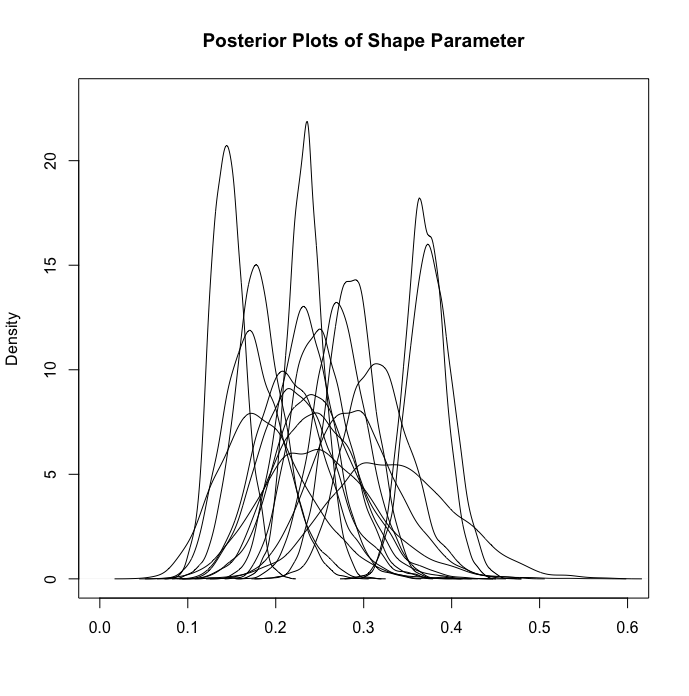
\includegraphics[width=8cm, height=7cm]{shapePostPlot}
  \caption{Posterior Plots of Weibull Shape Parameter}
  \label{Shape}
\end{figure}

\begin{figure}[ht]
\centering
\begin{subfigure}{.45\textwidth}
  \centering
  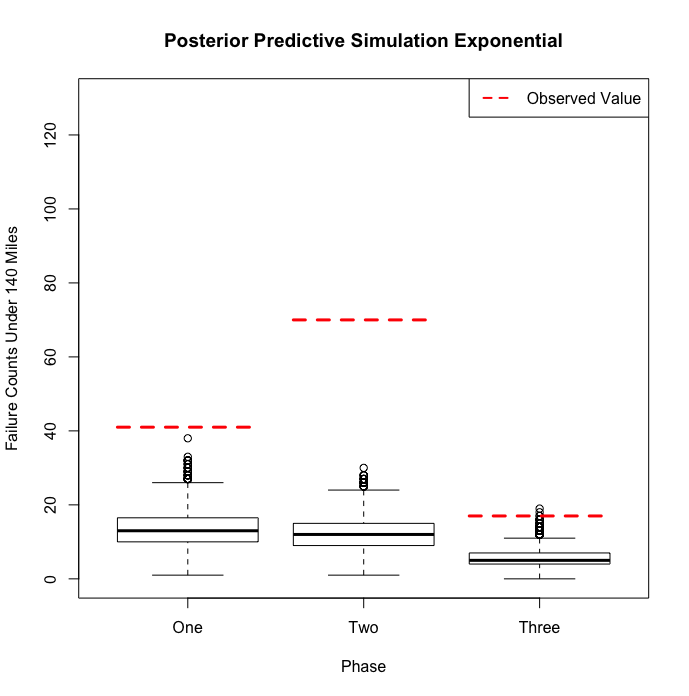
\includegraphics[width=.8\linewidth]{PPExpo}
\end{subfigure}%
\begin{subfigure}{.45\textwidth}
  \centering
  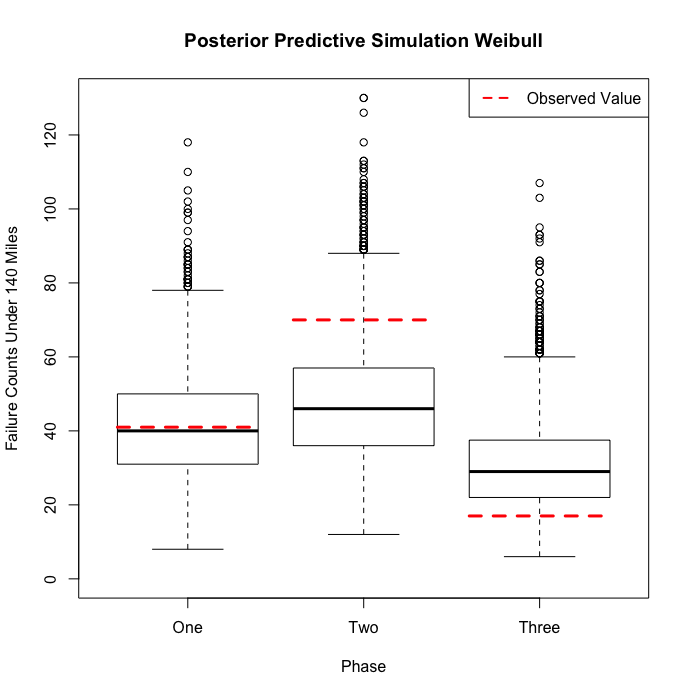
\includegraphics[width=.8\linewidth]{PPWeibull}
\end{subfigure}
\caption{Posterior Predictive Plots \\ Exponential vs. Weibull}
\label{fig:test}
\end{figure}

\begin{figure}[ht]
\centering
\begin{subfigure}{.5\textwidth}
  \centering
      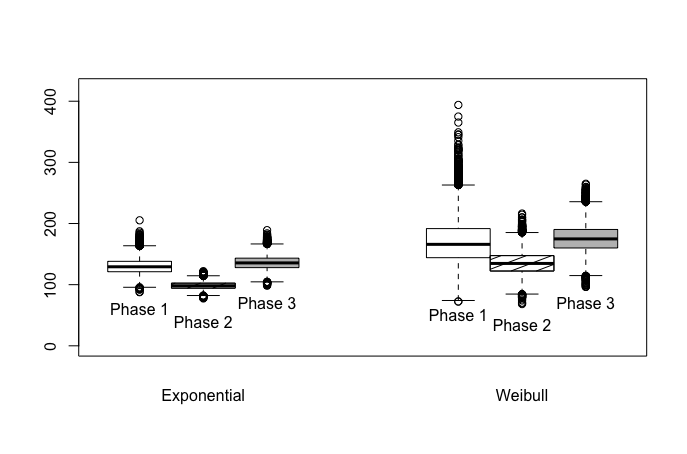
\includegraphics[width=8cm, height=7cm]{Boxplots}
  % \caption{Comparing EMTF for Different Models}
  %\label{fig:sub1}
\end{subfigure}%
\begin{subfigure}{.5\textwidth}
  \center
  \begin{tabular}{|c|c|c|c|c|}
  \multicolumn{5}{c}{\textbf{Summary Statistics}} \\
  \cline{1-5}
  Model & Phase & Mean & 90\% CI & 90\% CI \\
   & & & Low & Up \\
  \hline
  Expo & P1   & 129.98   & 110.22 &  152.23 \\
  Expo & P2   & 98.44  & 89.00 &  108.38  \\
  Expo & P3   & 135.89   & 117.78 &  155.45 \\
  Weibull & P1   & 169.96  & 116.95 & 236.16 \\
  Weibull & P2   & 135.24   & 104.89 & 167.48 \\
  Weibull & P3   & 175.51   & 138.87 & 214.23 \\
  \hline
  \end{tabular}
  %\label{fig:sub2}
\end{subfigure}
\caption{Comparing MMTF for Different Models}
\label{fig:MMTF Results}
\end{figure}

\begin{figure}[ht]
\centering
\begin{subfigure}{.5\textwidth}
  \centering
      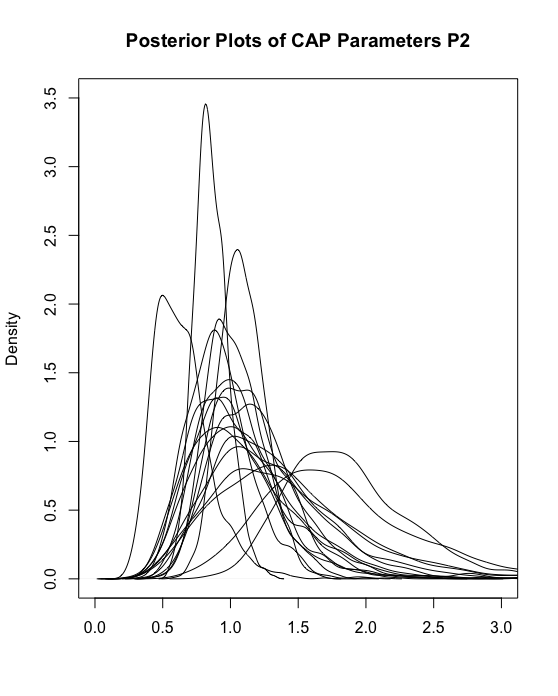
\includegraphics[width=8cm, height=7cm]{CAP2}
  % \caption{Corrective Action Period Parameters Posterior Distributions}
  %\label{fig:sub1}
\end{subfigure}%
\begin{subfigure}{.5\textwidth}
  \center
  	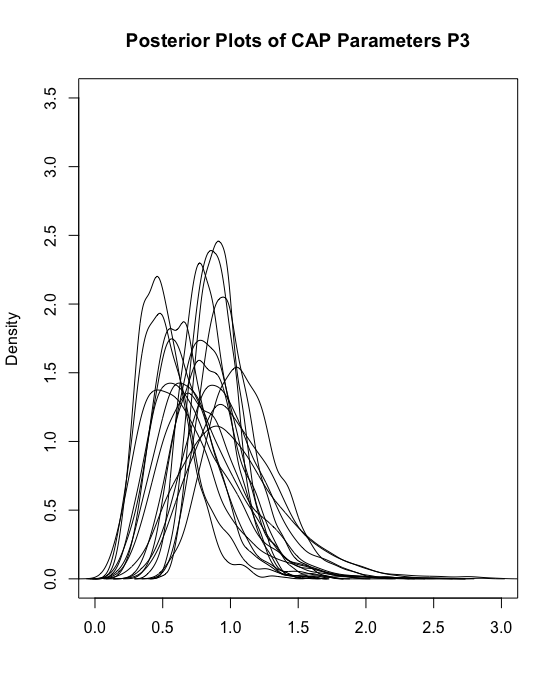
\includegraphics[width=8cm, height=7cm]{CAP3}
  %\label{fig:sub2}
\end{subfigure}
\caption{Posterior Distributions for Correction Parameters $\rho_{j}^{P2}$ and $\rho_{j}^{P3}$}
\label{fig:CAP}
\end{figure}

\end{document}
